\documentclass[10pt,handout]{beamer}

\usepackage[french]{babel}
\usepackage[utf8]{inputenc} 
\usepackage[T1]{fontenc}
\usepackage{lmodern}
\usepackage{beamerthemebars}
\usepackage{multicol}
\usepackage{pythontex}
\usepackage{amsmath}
\usepackage{graphics}
\usepackage{hyperref}
\usepackage{multimedia}
\usepackage{tikz}
\usetikzlibrary{calc}
\usetikzlibrary{fpu}
\usetikzlibrary{arrows.meta}
\usetikzlibrary{angles,quotes}
\usetikzlibrary{decorations.pathmorphing,patterns}
\usetikzlibrary{datavisualization.formats.functions}
%\usepackage[french]{babel}
\usepackage{pgfplots}
\pgfplotsset{compat=1.15}
\usepackage{mathrsfs}
\usetikzlibrary{arrows}
\usepackage{latexsym} % Símbolos                        ı
\usepackage{amsmath}
\usepackage{amssymb}
%%%%%%%%%%%%%%%%%%%%%%%%%%%%%%%
\usepackage{tikz-3dplot}
\usepackage[outline]{contour} % glow around text
\usepackage{xcolor}
\usepackage{listings}

\definecolor{codegreen}{rgb}{0,0.6,0}
\definecolor{codegray}{rgb}{0.5,0.5,0.5}
\definecolor{codepurple}{rgb}{0.58,0,0.82}
\definecolor{backcolour}{rgb}{0.95,0.95,0.92}

\lstdefinestyle{mystyle}{
    backgroundcolor=\color{backcolour},   
    commentstyle=\color{codegreen},
    keywordstyle=\color{magenta},
    numberstyle=\tiny\color{codegray},
    stringstyle=\color{codepurple},
    basicstyle=\ttfamily\footnotesize,
    breakatwhitespace=false,         
    breaklines=true,                 
    captionpos=b,                    
    keepspaces=true,                 
    numbers=left,                    
    numbersep=5pt,                  
    showspaces=false,                
    showstringspaces=false,
    showtabs=false,                  
    tabsize=2
}

\lstset{style=mystyle}

\colorlet{veccol}{green!50!black}
\colorlet{projcol}{blue!70!black}
\colorlet{myblue}{blue!80!black}
\colorlet{myred}{red!90!black}
\colorlet{mydarkblue}{blue!50!black}
\tikzset{>=latex} % for LaTeX arrow head
\tikzstyle{proj}=[projcol!80,line width=0.08] %very thin
\tikzstyle{area}=[draw=veccol,fill=veccol!80,fill opacity=0.6]
\tikzstyle{vector}=[-stealth,myblue,thick,line cap=round]
\tikzstyle{unit vector}=[->,veccol,thick,line cap=round]
\tikzstyle{dark unit vector}=[unit vector,veccol!70!black]
\usetikzlibrary{angles,quotes} % for pic (angle labels)
\contourlength{1.3pt}
\usetikzlibrary{decorations.pathreplacing}
%%%%%%%%%%%%%%%%%%%%%%%%%%%%%%%
\theoremstyle{plain} % default
  \newtheorem{thm}{Th\'eor\`eme}
\theoremstyle{definition}
  \newtheorem{defn}{D\'efinition}
\theoremstyle{example}
  \newtheorem{exmp}{Exemple}
\theoremstyle{example}
  \newtheorem{problema}{Probl\'eme}
\theoremstyle{remark}
  \newtheorem{respuesta}{R\'eponse}
\theoremstyle{remark}
  \newtheorem{rem}{Note}
%%%%%%%%%%%%%%%%%%%%%%%%%%%%
%\frenchdecimal{.}
%\useoutertheme{infolines}
%\usetheme{Marburg}
\setbeamercovered{transparent}

\title{Redes Neuronales}
\author{Antonio Falc\'o y Juan Pardo}
\date{Introducción a la Inteligencia Artificial} 

\begin{document}

\frame[plain]{%
\maketitle
}

%\begin{frame}
%  \tableofcontents
%\end{frame}

%\section{Contexto}
\frame[plain]{%
  \frametitle{Aprendizaje}  
  \framesubtitle{Una breve introducción al concepto de aprendizaje y a la inteligencia artificial en el campo del diseño de producto y de los procesos de fabricación.}
  \begin{block}{El proceso de aprendizaje}
    El aprendizaje es el proceso de adquisición de conocimientos, habilidades y actitudes a través de la experiencia, la instrucción y el estudio.
  \end{block}
  \begin{block}{El aprendizaje en la inteligencia artificial}
    En el campo de la inteligencia artificial, el aprendizaje es el proceso de \textcolor{red}{entrenar con un ordenador un modelo matemático  alimentado con datos para realizar una tarea específica}, como reconocer patrones en datos, tomar decisiones o predecir resultados.
\end{block}
\begin{block}{El proceso de aprendizaje con imágenes digitales}
  En el campo del procesamiento de imágenes digitales, el aprendizaje es el proceso de \textcolor{red}{entrenar con un ordenador un modelo matemático  alimentado con datos para analizar y procesar imágenes digitales}, como reconocer objetos, segmentar regiones de interés o mejorar la calidad de las imágenes.
\end{block}
%\py{2+2}
}

\frame[plain]{%
  \frametitle{Aprendizaje}  
  \framesubtitle{El esquema del proceso de aprendizaje máquina.}
\begin{center}
  \begin{tikzpicture}
    \node[draw] at (0,1) {\textcolor{blue}{Entrenamiento = Aprendizaje}};
    \node (A) at (0,0) {Datos = (Imágenes,Etiquetas)};
    \node[draw] (B) at (-6,-0.8) {\textcolor{red}{Modelo}};
    \node (C) at (-4,-0.8) {Imágenes};
    \node (D) at (0,-0.8) {Etiquetas};
    \node (E) at (-4,-3) {Imágenes};
    \node (F) at (0,-3) {Etiquetas};
    \node at (-5,-0.8) {$\times$};
    \draw[<-] (A)  (B) (D) -- (C);
    \node[draw] at (-2,-1.5) {\textcolor{red}{Procedimiento = Algoritmo}};
    \node[draw] at (0,-2.3) {\textcolor{blue}{Modelo Entrenado}};
    \draw[->] (E) -- (F);
  \end{tikzpicture}
\end{center}
\begin{itemize}
\item El proceso de \textcolor{blue}{aprendizaje = entrenamiento} lleva consigo la construcción de un modelo matemático que es alimentado con datos (imágenes y etiquetas) para realizar una tarea específica, como reconocer objetos en imágenes, segmentar regiones de interés o mejorar la calidad de las imágenes. 
\item La construcción del modelo se realiza empleando un \textcolor{red}{procedimiento = algoritmo}.
\end{itemize}
}

\frame[plain]{%
  \frametitle{Problemas clave}  
  %\framesubtitle{}
\centering
  \begin{enumerate}
    \item \textbf{Representación de datos}: La representación de datos es un desafío importante, ya que los \textcolor{red}{datos} pueden ser complejos y difíciles de analizar.
    
    \item \textbf{Optimización}: La optimización es un problema clave en la inteligencia artificial, ya que muchos \textcolor{red}{algoritmos} buscan encontrar las mejores soluciones entre múltiples opciones.

    \item \textbf{Escalabilidad}: La escalabilidad se refiere a la capacidad de los \textcolor{red}{algoritmos} para manejar grandes cantidades de datos y hacer predicciones precisas en tiempo real.

    \item \textbf{Interpretabilidad}: La interpretabilidad es el problema de entender cómo los \textcolor{red}{algoritmos} llegan a sus conclusiones y por qué toman ciertas decisiones.

    \item \textbf{Robustez}: La robustez se refiere a la capacidad de los \textcolor{red}{algoritmos} para funcionar correctamente en diferentes condiciones y ambientes.

    \item \textbf{Explicabilidad}: La explicabilidad es el problema de justificar las decisiones tomadas por los \textcolor{red}{algoritmos} y cómo se relacionan con los \textcolor{red}{datos} de entrada.
  
    \item \textbf{Equidad}: La equidad se refiere a la capacidad de los \textcolor{red}{algoritmos} para tomar decisiones no discriminatorias y respetuosas con los derechos humanos.
  \end{enumerate}
}

\frame[plain]{%
  \frametitle{Ejemplo de una red neuronal simple}  
  %\framesubtitle{}
    %\centering
  \textbf{Objetivo}: Diseñar una red neuronal simple que pueda predecir si tipo de flor es \emph{Iris setosa} a partir de la anchura y la longitud (cm) del pétalo de una flor \emph{Iris}.
  \begin{center}
    \begin{tikzpicture}
      \node[draw] at (0,1) {\textcolor{blue}{Entrenamiento = Aprendizaje}};
      \node (A) at (0,0) {Datos = ((Anchura,Longitud),Tipo)};
      \node[draw] (B) at (-6.5,-0.8) {\textcolor{red}{Modelo}};
      \node (C) at (-4,-0.8) {(Anchura,Longitud)};
      \node (D) at (0,-0.8) {Tipo};
      \node (E) at (-4,-3) {(Anchura,Longitud)};
      \node (F) at (0,-3) {Tipo};
      \node at (-5.6,-0.8) {$\times$};
      \draw[<-] (A)  (B) (D) -- (C);
      \node[draw] at (-2,-1.5) {\textcolor{red}{Procedimiento = Algoritmo}};
      \node[draw] at (0,-2.3) {\textcolor{blue}{Modelo Entrenado}};
      \draw[->] (E) -- (F);
    \end{tikzpicture}
\end{center}
    \textcolor{red}{Modelo}: $\text{Tipo} = \sigma\left(\textcolor{blue}{w_1} \times \text{Anchura} + \textcolor{blue}{w_2} \times \text{Longitud}  + \textcolor{blue}{b_1}\right) = \left\{ 
      \begin{array}{ll}
        0 & \text{si } \text{Tipo} = \text{Iris setosa} \\
        1 & \text{si } \text{Tipo} \neq \text{Iris setosa}
      \end{array}
    \right.$
}

\frame[plain]{%
  \frametitle{Modelo del perceptrón}  
  \centering
\begin{tikzpicture}[shorten >=1pt,->]
  \tikzstyle{unit}=[draw,shape=circle,minimum size=1.15cm]
  \node[draw] at (1,2.3) {$w_1$};
  \node[draw] at (1,0) {$w_2$};
  \node[unit](p) at (2,1){Tipo};
  %\node(dots) at (-0.25,1){\vdots};
  \draw (0,2.5)  node[xshift=-5]{Anchura} -- (p);
  \draw (0,1.25) node[xshift=-5]{$b_1$} --(p);
  \draw (0,0) node[xshift=-10]{Longitud} -- (p);
  \draw (p) -- (3,1) node[xshift=30]{Tipo $:= \sigma(z)$};
\end{tikzpicture}
}

\frame[plain]{%
  \frametitle{Modelo del perceptrón}  
  %\framesubtitle{}
\begin{center}
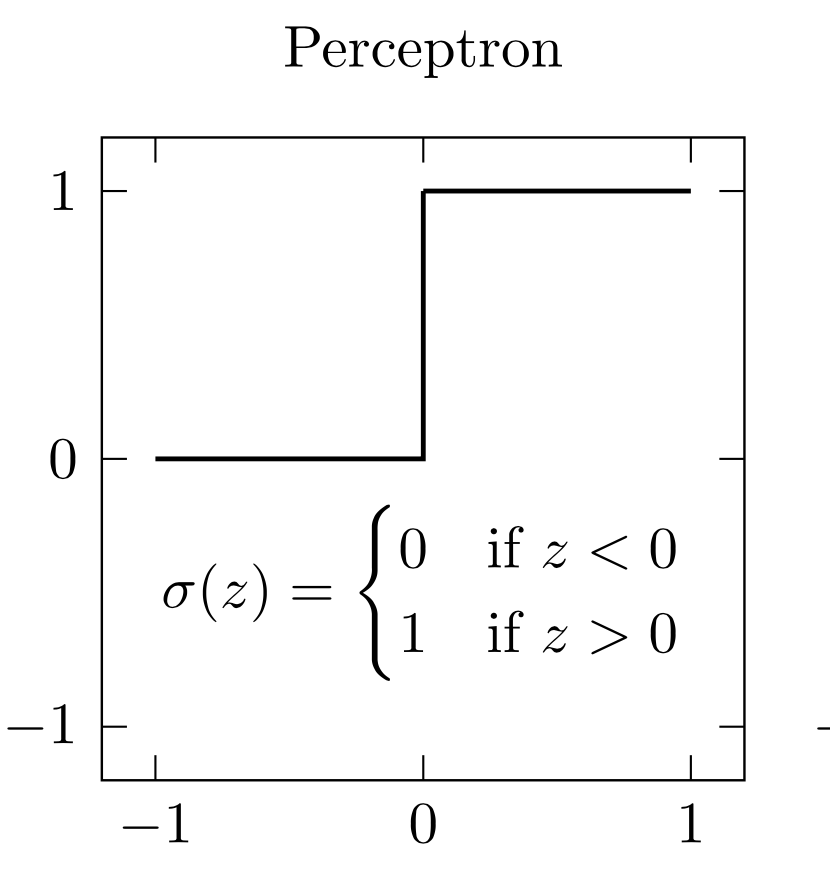
\includegraphics[width=0.3\textwidth]{Figura01.png}
\end{center}
Consideramos la función de activación que caracteriza el tipo 
de flor \emph{Iris setosa} como 
$$
\sigma(z) = \left\{ 
  \begin{array}{ll}
    0 \, (\text{\emph{Iris setosa}}) & \text{si } z < 0 \\
    1 \, (\text{\emph{No Iris setosa}}) & \text{si } z > 0
  \end{array}
\right.
$$
y tomamos 
$$
z = \textcolor{blue}{w_1} \times \text{Anchura} + \textcolor{blue}{w_2} \times \text{Longitud}  + \textcolor{blue}{b_1}
$$
La caracterización del modelo de perceptrón se reduce al conocimiento de los parámetros $\textcolor{blue}{w_1}$, $\textcolor{blue}{w_2}$ (pesos) y $\textcolor{blue}{b_1}$ (sesgo).
}



\frame[plain]{%
  \frametitle{Modelo del perceptrón}  
  %\framesubtitle{}
  \begin{center}
    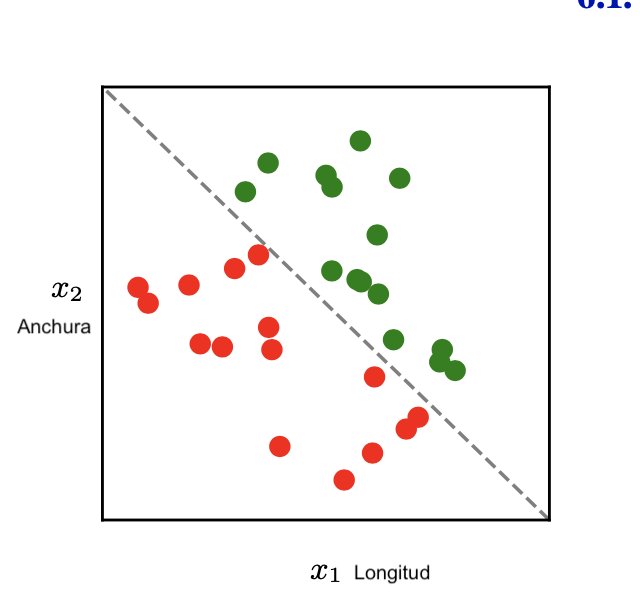
\includegraphics[width=0.4\textwidth]{Figura02.png}
    \end{center}
La separación de las flores \emph{Iris setosa} y \emph{No Iris setosa} se caracteriza empleando la ecuación
$$
z = \textcolor{blue}{w_1} \times \text{Anchura (cm)} + \textcolor{blue}{w_2} \times \text{Longitud (cm)}  + \textcolor{blue}{b_1} = 0
$$
en la imagen se representa con la línea discontinua.
}

\frame[plain]{%
  \frametitle{Modelo del perceptrón: Aprendizaje computacional}  
  %\framesubtitle{}
\textbf{Objetivo:} Tenemos que calcular los parámetros $\textcolor{blue}{w_1}$, $\textcolor{blue}{w_2}$ y $\textcolor{blue}{b_1}$ que caracterizan el modelo de perceptrón. Para ello, empleamos el algoritmo de aprendizaje computacional que se basa en la minimización de la función de coste siguiente:
\begin{itemize}
\item Tomamos un conjunto de datos de entrenamiento 
$$\{(x^{(1)},y^{(1)}),\ldots,(x^{(m)},y^{(m)})\},$$ donde $x^{(i)} = (x_1^{(i)},x_2^{(i)}),$ siendo 
$x_1^{(i)} = \text{ Longitud }$ y $x_2^{(i)} = \text{ Anchura },$ es el vector de características de la $i$-ésima flor de la base de datos y $y^{(i)} \in \{0,1\}$ es la etiqueta correspondiente. 
\item La función de coste se puede definir como:
$$
\frac{1}{m}\sum_{i=1}^m (y^{(i)} -\sigma(z^{(i)}))^2 = \frac{1}{m}\sum_{i=1}^m (y^{(i)}-\sigma(\textcolor{blue}{w_1} \times x_1^{(i)} + \textcolor{blue}{w_2} \times x_2^{(i)} + \textcolor{blue}{b_1}))^2,
$$
\end{itemize}
}

\frame[plain]{%
  \frametitle{Modelo del perceptrón: Aprendizaje computacional}  
  %\framesubtitle{}
\begin{itemize}
\item Analicemos La función de coste:
$$
0 \le \frac{1}{m}\sum_{i=1}^m (y^{(i)}-\sigma(\textcolor{blue}{w_1} \times x_1^{(i)} + \textcolor{blue}{w_2} \times x_2^{(i)} + \textcolor{blue}{b_1}))^2 \le 1,
$$
En el caso de que $y^{(i)} \neq \sigma(z^{(i)}),$ para todos los datos de entrenamiento la función de coste tomaría el valor de $1$ y $0$ cuando $y^{(i)} = \sigma(z^{(i)}).$ 
\item Supongamos fijados los valores de $\textcolor{blue}{w_1},\textcolor{blue}{w_2}$ y 
$\textcolor{blue}{b_1},$ y observemos que cada vez que nos equivocamos en la predicción, la función de coste aumenta una cantidad $1/m,$ luego el valor de la función de coste nos indica el porcentaje de errores en la predicción:
$$
\frac{\text{Cantidad de errores en la predicción}}{\text{Número total de datos de entrenamiento}}(\textcolor{blue}{w_1},\textcolor{blue}{w_2},\textcolor{blue}{b_1}).
$$
\end{itemize}
}

\frame[plain]{%
  \frametitle{Modelo del perceptrón: Aprendizaje computacional}  
  %\framesubtitle{}
\begin{itemize}
\item Nuestro objetivo es minimizar la función de coste:
$$
\min_{\textcolor{blue}{w_1},\textcolor{blue}{w_2},\textcolor{blue}{b_1}} \frac{\text{Cantidad de errores en la predicción}}{\text{Número total de datos de entrenamiento}}(\textcolor{blue}{w_1},\textcolor{blue}{w_2},\textcolor{blue}{b_1}),
$$
esto es, minimizar el porcentaje de errores en la predicción para los datos de entrenamiento:
$$
\min_{\textcolor{blue}{w_1},\textcolor{blue}{w_2},\textcolor{blue}{b_1}} \frac{1}{m}\sum_{i=1}^m (y^{(i)}-\sigma(\textcolor{blue}{w_1} \times x_1^{(i)} + \textcolor{blue}{w_2} \times x_2^{(i)} + \textcolor{blue}{b_1}))^2.
$$
\item El resultado de este proceso de minimización nos proporcionará los valores de los parámetros $\textcolor{blue}{\widehat{w}_1},\textcolor{blue}{\widehat{w}_2},\textcolor{blue}{\widehat{b}_1}$ que caracterizan el modelo de perceptrón.
\end{itemize}
}



\frame[plain]{%
  \frametitle{Modelo entrenado del perceptrón}  
  %\framesubtitle{}
\begin{itemize}
\item El modelo entrenado de perceptrón viene dado por la función::
$$
\textcolor{blue}{\text{Mod. Entr.}}(\text{Longitud},\text{Anchura})=\sigma(\textcolor{blue}{\widehat{w}_1} \times \text{Longitud} + \textcolor{blue}{\widehat{w}_2} \times \text{Anchura} + \textcolor{blue}{\widehat{b}_1}).
$$
\item Podemos emplear un segundo conjunto de datos de prueba para evaluar la precisión del modelo entrenado.
\end{itemize}
}


\begin{frame}[fragile]
  Este proyecto requiere Python 3.7 o superior, Scikit-Learn 1.0.1 o superior y TensorFlow 2.8.0 o superior.:
\frametitle{Código Python}
\begin{lstlisting}[language=Python]
  import sys
  assert sys.version_info >= (3, 7)
  from packaging import version
  import sklearn
  assert version.parse(sklearn.__version__) >= version.parse("1.0.1")
  import tensorflow as tf
  assert version.parse(tf.__version__) >= version.parse("2.8.0")
\end{lstlisting}  
\begin{pycode}
import sys
assert sys.version_info >= (3, 7)
from packaging import version
import sklearn
assert version.parse(sklearn.__version__) >= version.parse("1.0.1")
import tensorflow as tf
assert version.parse(tf.__version__) >= version.parse("2.8.0")
\end{pycode}  
\end{frame}

\begin{frame}[fragile]
Definimos las fuentes para tener una mejor visualización de los gráficos:
\frametitle{Código Python}
\begin{lstlisting}[language=Python]
  import matplotlib.pyplot as plt
  plt.rc('font', size=14)
  plt.rc('axes', labelsize=14, titlesize=14)
  plt.rc('legend', fontsize=14)
  plt.rc('xtick', labelsize=10)
  plt.rc('ytick', labelsize=10)
\end{lstlisting}  
\begin{pycode}
import matplotlib.pyplot as plt
plt.rc('font', size=14)
plt.rc('axes', labelsize=14, titlesize=14)
plt.rc('legend', fontsize=14)
plt.rc('xtick', labelsize=10)
plt.rc('ytick', labelsize=10)
\end{pycode}  
\end{frame}


\begin{frame}[fragile]
  Creamos un directorio para guardar las imágenes generadas:
  \frametitle{Código Python}
  \begin{lstlisting}[language=Python]
from pathlib import Path
IMAGES_PATH = Path()/"images"/"ann"
IMAGES_PATH.mkdir(parents=True, exist_ok=True)
    
def save_fig(fig_id, tight_layout=True,fig_extension="png", resolution=300):
  path = IMAGES_PATH / f"{fig_id}.{fig_extension}"
  if tight_layout:
      plt.tight_layout()
  plt.savefig(path, format=fig_extension, dpi=resolution)
  \end{lstlisting}  
  \begin{pycode}
from pathlib import Path
IMAGES_PATH = Path()/"images"/"ann"
IMAGES_PATH.mkdir(parents=True, exist_ok=True)

def save_fig(fig_id, tight_layout=True, fig_extension="png", resolution=300):
  path = IMAGES_PATH/f"{fig_id}.{fig_extension}"
  if tight_layout:
    plt.tight_layout()
  plt.savefig(path,format=fig_extension, dpi=resolution)
  \end{pycode}  
  \end{frame}


\begin{frame}[fragile]
Definimos el perceptron:
\frametitle{Código Python}
\begin{lstlisting}[language=Python]
import numpy as np
from sklearn.datasets import load_iris
from sklearn.linear_model import Perceptron

iris = load_iris(as_frame=True)
X = iris.data[["petal length (cm)", "petal width (cm)"]].values
y = (iris.target == 0)  # Iris setosa

per_clf = Perceptron(random_state=42)
per_clf.fit(X, y)
    \end{lstlisting}  
    \begin{pycode}
import numpy as np
from sklearn.datasets import load_iris
from sklearn.linear_model import Perceptron

iris = load_iris(as_frame=True)
X = iris.data[["petal length (cm)", "petal width (cm)"]].values
y = (iris.target == 0)  # Iris setosa

per_clf = Perceptron(random_state=42)
per_clf.fit(X, y)
\end{pycode}  
\end{frame}

\begin{frame}[fragile]
Empleamos el modelo para determinar si las flores son de tipo \emph{Iris setosa} o no:
\frametitle{Código Python}
\begin{lstlisting}[language=Python]
X_new = [[2, 0.5], [3, 1]]
y_pred = per_clf.predict(X_new)  # predice True y False para  estas 2 flores

print(y_pred)
    \end{lstlisting}  
    \begin{pycode}
X_new = [[2, 0.5], [3, 1]]
y_pred = per_clf.predict(X_new)  # predice True y False para  estas 2 flores

print(y_pred)
\end{pycode}  
\end{frame}



\begin{frame}[fragile]
  El `Perceptrón` es equivalente a un `SGDClassifier` con `loss="perceptron"`, sin regularización y una tasa de aprendizaje constante igual a 1:
\frametitle{Código Python}
\begin{lstlisting}[language=Python]
# codigo extra - muestra como construir y entrenar un Perceptron
from sklearn.linear_model import SGDClassifier
    
sgd_clf = SGDClassifier(loss="perceptron", penalty=None,learning_rate="constant", eta0=1, random_state=42)
sgd_clf.fit(X, y)
assert (sgd_clf.coef_ == per_clf.coef_).all()
assert (sgd_clf.intercept_ == per_clf.intercept_).all()
print(sgd_clf.predict([[2, 0.5], [3, 1]]))
      \end{lstlisting}  
\begin{pycode}
from sklearn.linear_model import SGDClassifier
    
sgd_clf = SGDClassifier(loss="perceptron", penalty=None,learning_rate="constant", eta0=1, random_state=42)
sgd_clf.fit(X, y)
assert (sgd_clf.coef_ == per_clf.coef_).all()
assert (sgd_clf.intercept_ == per_clf.intercept_).all()
print(sgd_clf.predict([[2, 0.5], [3, 1]]))
\end{pycode}  
\end{frame}

\begin{frame}[fragile]
Cuando el perceptrón encuentra un límite de decisión que separa adecuadamente las clases, deja de aprender. Esto significa que el límite de decisión suele estar bastante cerca de una clase:
\frametitle{Código Python}
\begin{lstlisting}[language=Python]
# extra code - plots the decision boundary of a Perceptron on the iris dataset

import matplotlib.pyplot as plt
from matplotlib.colors import ListedColormap

a = -per_clf.coef_[0, 0] / per_clf.coef_[0, 1]
b = -per_clf.intercept_ / per_clf.coef_[0, 1]
axes = [0, 5, 0, 2]
x0, x1 = np.meshgrid(
    np.linspace(axes[0], axes[1], 500).reshape(-1, 1),
    np.linspace(axes[2], axes[3], 200).reshape(-1, 1),
)
X_new = np.c_[x0.ravel(), x1.ravel()]
y_predict = per_clf.predict(X_new)
zz = y_predict.reshape(x0.shape)
custom_cmap = ListedColormap(['#9898ff', '#fafab0'])
\end{lstlisting}  
\begin{pycode}
# extra code – plots the decision boundary of a Perceptron on the iris dataset

import matplotlib.pyplot as plt
from matplotlib.colors import ListedColormap

a = -per_clf.coef_[0, 0] / per_clf.coef_[0, 1]
b = -per_clf.intercept_ / per_clf.coef_[0, 1]
axes = [0, 5, 0, 2]
x0, x1 = np.meshgrid(
    np.linspace(axes[0], axes[1], 500).reshape(-1, 1),
    np.linspace(axes[2], axes[3], 200).reshape(-1, 1),
)
X_new = np.c_[x0.ravel(), x1.ravel()]
y_predict = per_clf.predict(X_new)
zz = y_predict.reshape(x0.shape)
custom_cmap = ListedColormap(['#9898ff', '#fafab0'])

plt.figure(figsize=(7, 3))
plt.plot(X[y == 0, 0], X[y == 0, 1], "bs", label="No Iris setosa")
plt.plot(X[y == 1, 0], X[y == 1, 1], "yo", label="Iris setosa")
plt.plot([axes[0], axes[1]], [a * axes[0] + b, a * axes[1] + b], "k-",
         linewidth=3)
plt.contourf(x0, x1, zz, cmap=custom_cmap)
plt.xlabel("Longitud del pétalo (cm)")
plt.ylabel("Anchura del pétalo (cm)")
plt.legend(loc="lower right")
plt.axis(axes)
plt.show()
\end{pycode}  
\end{frame}

\begin{frame}[fragile]
  \frametitle{Código Python}
\begin{lstlisting}[language=Python]
plt.figure(figsize=(7, 3))
plt.plot(X[y == 0, 0], X[y == 0, 1], "bs", label="No Iris setosa")
plt.plot(X[y == 1, 0], X[y == 1, 1], "yo", label="Iris setosa")
plt.plot([axes[0], axes[1]], [a * axes[0] + b, a * axes[1] + b], "k-",
         linewidth=3)
plt.contourf(x0, x1, zz, cmap=custom_cmap)
plt.xlabel("Longitud del petalo (cm)")
plt.ylabel("Anchura del petalo (cm)")
plt.legend(loc="lower right")
plt.axis(axes)
plt.show()
\end{lstlisting}  
\begin{pycode}
\end{pycode}  
\end{frame}

\frame[plain]{%
  \frametitle{Figura}  
  %\framesubtitle{}
\centering

\includegraphics[width=0.7\textwidth]{Figure_1.png}
}

\frame[plain]{%
  \frametitle{Funciones de activación}  
  %\framesubtitle{}
\begin{itemize}
\item Un parámetro más de este tipo de modelos es la elección de la \textcolor{blue}{función de activación}. La función de activación es una función matemática que se aplica a la salida de cada neurona en la red neuronal. 
\item En el caso particular del perceptrón, la función de activación es la función de Heaviside:
$$
\sigma(z) = H(z) = \left\{ 
  \begin{array}{ll}
    0 & \text{si } z < 0, \\
    1 & \text{si } z > 0.
  \end{array}
  \right.
$$
\item Otras funciones comunmente empleadas son la función sigmoide, la función tangente hiperbólica y la función ReLU:
$$
\sigma(z) = \frac{1}{1+e^{-z}}, \quad \sigma(z) = \tanh(z), \quad \sigma(z) = \max(0,z).
$$
Recordar que $$\tanh(z)=\frac{e^{z}-e^{-z}}{e^{z}+e^{-z}}$$
\end{itemize}
}

\frame[plain]{%
  \frametitle{Figura}  
  %\framesubtitle{}
\centering

\includegraphics[width=1\textwidth]{Figure_2.png}
}

\frame[plain]{%
  \frametitle{Funciones de coste}  
  %\framesubtitle{}
\begin{itemize}
\item Otro parámetro más de este tipo de modelos es la elección de la \textcolor{blue}{función de coste}. La función de coste es una función matemática que se emplea para medir la diferencia entre la salida predicha por el modelo y la salida real de los datos de entrenamiento.
\item En nuestro caso, la función de coste es la función de coste cuadrático medio:
$$
\frac{1}{m}\sum_{i=1}^m (y^{(i)}-\sigma(\textcolor{blue}{w_1} \times x_1^{(i)} + \textcolor{blue}{w_2} \times x_2^{(i)} + \textcolor{blue}{b_1}))^2
$$
\item La función que relaciones los datos de entrada con la salida que deseamos predecir se denomina \textcolor{blue}{función de hipótesis} y la denotamos por $z = \phi_{\text{modelo}}(x_1,x_2)$: 
\item La red neuronal se puede ver como una función $z = \phi_{\textcolor{blue}{(w_1,w_2,b_1)}}^{\sigma}(x_1,x_2) =\sigma(\textcolor{blue}{w_1} \times x_1 + \textcolor{blue}{w_2} \times x_2 + \textcolor{blue}{b_1}).$
\end{itemize}
}

\frame[plain]{%
  \frametitle{Funciones de coste}  
  %\framesubtitle{}
\begin{itemize}
\item Podemos entonces escribir la función de pérdida como:
$$
\frac{1}{m}\sum_{i=1}^m (\phi_{\text{modelo}}(x_1^{(i)},x_2^{(i)})-\phi_{\textcolor{blue}{(w_1,w_2,b_1)}}^{\sigma}(x_1^{(i)},x_2^{(i)}))^2 
$$
\item Aunque se pueden en general definir funciones de coste más complejas, la función de coste cuadrático medio es una de las más comunes en la práctica.
\item La elección de la función de coste es un aspecto importante en el diseño de un modelo de red neuronal, ya que afecta a la forma en que el modelo aprende de los datos de entrenamiento.
\item En general una función de pérdida se puede escribir como:
$$
\mathcal{L}(\phi_{\text{modelo}}(x_1,x_2),\phi_{\textcolor{blue}{(w_1,w_2,b_1)}}^{\sigma}(x_1,x_2),\text{Datos Entrenamiento}).
$$
\item Con una notación más compacta, la función de pérdida se puede escribir como:  
$$
\mathcal{L}(\textbf{y},\phi_{\textcolor{blue}{\boldsymbol{\theta}}}^{\sigma}(\mathbf{x})),
$$
donde $(\mathbf{x},\mathbf{y})$ son datos del conjunto de entrenamiento y $\boldsymbol{\theta}$ son los parámetros del modelo.
\end{itemize}
}

\frame[plain]{%
  \frametitle{Funciones de coste}  
  %\framesubtitle{}
\begin{itemize}
\item Con una notación más compacta, la función de pérdida se puede escribir como:  
$$
\mathcal{L}(\textbf{y},\phi_{\textcolor{blue}{\boldsymbol{\theta}}}^{\sigma}(\mathbf{x})),
$$
donde $(\mathbf{x},\mathbf{y})$ son datos del conjunto de entrenamiento y $\boldsymbol{\theta}$ son los parámetros del modelo.
\item El modelo que obtenemos al minimizar la función de pérdida se denomina \textcolor{blue}{modelo entrenado} y formalmente se representa por 
$$
\mathbf{y} = \phi_{\textcolor{blue}{\widehat{\boldsymbol{\theta}}}}^{\sigma}(\mathbf{x})
$$
donde $\widehat{\boldsymbol{\theta}}$ son los parámetros del modelo entrenado que formalmente se obtienen al resolver el problema de optimización:
$$
\widehat{\boldsymbol{\theta}} = \arg\min_{\boldsymbol{\theta}} \mathcal{L}(\textbf{y},\phi_{\textcolor{blue}{\boldsymbol{\theta}}}^{\sigma}(\mathbf{x})).
$$
\end{itemize}
}

\frame[plain]{%
  \frametitle{Modelos de Redes Neuronales}  
  %\framesubtitle{}
\begin{itemize}
\item Los modelos de redes neuronales son modelos matemáticos que se inspiran en la forma en que funcionan las neuronas en el cerebro humano.
\item La idea es la siguiente. Consideremos ahora un conjunto de datos de entrada $\mathbf{x} = (x_1,x_2,\ldots,x_n)$ y un conjunto de datos de salida $\mathbf{y} = (y_1,y_2,\ldots,y_m)$ \textbf{que representan objetos que podemos codificar empleando vectores numéricos}.
\end{itemize}
}

\frame[plain]{%
  \frametitle{Modelos de Redes Neuronales: Una capa}  
  %\framesubtitle{}
Se elige una función de activación $\sigma$ y se define la función de hipótesis $\phi_{\textcolor{blue}{\boldsymbol{\theta}}}^{\sigma}(\mathbf{x})$ como:
\begin{enumerate}
  \item Para cada par de datos $(\mathbf{x},\mathbf{y})$ del conjunto de entrenamiento, procedemos del modo siguiente:
  \item Escribimos $\mathbf{z}_0 := \mathbf{x},$ y consideramos como vector de parámetros $\boldsymbol{\theta}=(W_1,\mathbf{b}_1)$ del modelo una matriz de pesos $W_1$ y un vector de sesgos $\mathbf{b}_1$ siguiente:
$$
W_1 = \begin{bmatrix}
W_{11}^{(1)} & W_{12}^{(1)} & \cdots & W_{1n}^{(1)} \\
W_{21}^{(1)} & W_{22}^{(1)} & \cdots & W_{2n}^{(1)} \\
\vdots & \vdots & \ddots & \vdots \\
W_{m 1}^{(1)} & W_{N_1 2}^{(1)} & \cdots & W_{m n}^{(1)}
\end{bmatrix}, \quad \mathbf{b}_1 = \begin{bmatrix}
  b_1^{(1)} \\ b_2^{(1)} \\ \vdots \\ b_{m}^{(1)}
  \end{bmatrix},
$$
\end{enumerate}
}

\frame[plain]{%
  \frametitle{Modelos de Redes Neuronales: Una capa}  
  %\framesubtitle{}

 Calculamos un vector $\mathbf{z}_1$ del modo siguiente:
 $$
\mathbf{z}_1 =\sigma(W_1\mathbf{z}_0 + \mathbf{b}_1) := \begin{bmatrix}
\sigma(\sum_{j=1}^{n} W_{1j}^{(1)}x_j + b_1^{(1)}) \\
\sigma(\sum_{j=1}^{n} W_{2j}^{(1)}x_j + b_2^{(1)}) \\
\vdots \\
\sigma(\sum_{j=1}^{n} W_{m j}^{(1)}x_j + b_{m}^{(1)})
\end{bmatrix}
$$
El vector de salida $\mathbf{z}_1$ tiene el mismo número de componentes que el vector de etiquetas $\mathbf{y}.$ Podemos considerar $\mathbf{z}_1$ como un nuevo vector de características que se emplea para calcular la salida del modelo. El error cometido en la predicción se puede medir empleando:
$$
\|\mathbf{z}_1 - \mathbf{y}\|^2 := \sum_{i=1}^{m} \left(\sigma\left(\sum_{j=1}^{n} W_{i j}^{(1)}x_j + b_{j}^{(1)}\right)-y_i \right)^2.
$$
}

\frame[plain]{%
  \frametitle{Modelos de Redes Neuronales: Una capa}  
  %\framesubtitle{}
\begin{center}
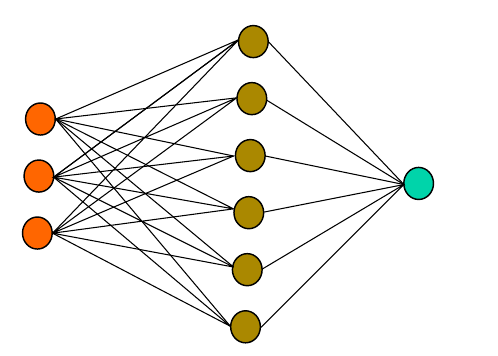
\includegraphics[width=0.7\textwidth]{Figura03.png}
\end{center}
En esta imagen representa una red neuronal de una capa con $n=3,$ es decir $\mathbf{x}=(x_1,x_2,x_3),$ y $m=6,$ es decir $\mathbf{y}=(y_1,y_2,y_3,y_4,y_5,y_6).$ En consecuencia la matriz $W_1$ tiene dimensión $6\times 3 = 18$ y el vector $\mathbf{b}_1$ tiene dimensión $6.$ Esto hace un total de $24$ parámetros que caracterizan el modelo.
}

\frame[plain]{%
  \frametitle{Modelos de Redes Neuronales: Una capa}  
  %\framesubtitle{}
La función de coste para un conjunto de entrenamiento
$$
(\mathbf{x}_1,\mathbf{y}_1), \ldots ,(\mathbf{x}_{\ell},\mathbf{y}_{\ell})
$$
donde para cada dato de entrada $\mathbf{x}_1,\mathbf{x}_2,\ldots,\mathbf{x}_{\ell}$ puedo calcular un vector de salida $\mathbf{z}_1^{(1)}, \mathbf{z}_1^{(2)},\ldots \mathbf{z}_1^{(\ell)}$ del modo siguiente:
$$
\begin{matrix}
\mathbf{z}_1^{(1)} & = \sigma(W_1\mathbf{x}_1 + \mathbf{b}_1),\\
\mathbf{z}_1^{(2)} & = \sigma(W_1\mathbf{x}_2 + \mathbf{b}_1), \\ 
\vdots & \vdots \\
\mathbf{z}_1^{(\ell)} & = \sigma(W_1\mathbf{x}_{\ell} + \mathbf{b}_1).
\end{matrix}
$$
se puede escribir para cada dato $\mathbf{x}_{i}=(x_1^{(i)},\ldots,x_{n}^{(i)})$ e $\mathbf{y}_i = (y_1^{(i)},\ldots,y_{m}^{(i)})$ con $1 \le i \le \ell,$ como
$$
\frac{1}{\ell} \sum_{i=1}^{\ell}\|\mathbf{z}_1^{(i)} - \mathbf{y}_i\|^2 = \frac{1}{\ell} \sum_{i=1}^{\ell}\sum_{j=1}^{m} \left(\sigma\left(\sum_{k=1}^{n} W_{j k}^{(1)} x_k^{(i)} + b_{j}^{(1)}\right)-y_j^{(i)} \right)^2.
$$
}

\frame[plain]{%
  \frametitle{Modelos de Redes Neuronales: Una capa}  
  %\framesubtitle{}
La función de coste para el conjunto de entrenamiento 
$$
\mathcal{L}(W_1,\mathbf{b}_1) = \frac{1}{\ell} \sum_{i=1}^{\ell}\sum_{j=1}^{m} \left(\sigma\left(\sum_{k=1}^{n} W_{j k}^{(1)} x_k^{(i)} + b_{j}^{(1)}\right)-y_j^{(i)} \right)^2
$$
depende de los parámetros $W_1$ y $\mathbf{b}_1.$ El objetivo es minimizar la función de coste $\mathcal{L}(W_1,\mathbf{b}_1)$ respecto a los parámetros $W_1$ y $\mathbf{b}_1.$ Una 
vez calculados los valores óptimos $(\widehat{W}_1,\widehat{b}_1)$
la función predicción se puede escribir como:
$$
\mathbf{y} = \phi_{\textcolor{blue}{\widehat{W}_1,\widehat{\mathbf{b}}_1}}^{\sigma}(\mathbf{x}) = \sigma(\widehat{W}_1\mathbf{x} + \widehat{\mathbf{b}}_1).
$$
}

\end{document}